\subsection{Three-Dimensional Tradeoff: Tag Length, Witness Cost, Distortion}

Recall from Section 2 that observer strategies are characterized by three dimensions:
\begin{itemize}
\item \textbf{Tag length} $L$: bits required to encode a type identifier ($L \geq \log_2 k$ for $k$ types)
\item \textbf{Witness cost} $W$: minimum number of primitive queries for type identity checking
\item \textbf{Distortion} $D$: probability of misclassification, $D = \Pr[\hat{C} \neq C]$.
\end{itemize}

We compare two observer classes:

\begin{definition}[Interface-only observer]
An observer that queries only interface membership ($q_I \in \Phi_{\mathcal{I}}$), with no access to explicit type tags.
\end{definition}

\begin{definition}[Nominal-tag observer]
An observer that may read a single type identifier (nominal tag) per value, in addition to interface queries.
\end{definition}

\begin{theorem}[Pareto Optimality of Nominal-Tag Observers]\label{thm:lwd-optimal}
In any information-barrier domain, nominal-tag observers achieve the unique Pareto-optimal point in the $(L, W, D)$ space with $D = 0$:
\begin{itemize}
\item \textbf{Tag length}: $L = \lceil \log_2 k \rceil$ bits for $k$ types
\item \textbf{Witness cost}: $W = O(1)$ queries (one tag read)
\item \textbf{Distortion}: $D = 0$ (zero misclassification probability)
\end{itemize}

In such domains, interface-only observers achieve:
\begin{itemize}
\item \textbf{Tag length}: $L = 0$ bits (no explicit tag)
\item \textbf{Witness cost}: $W = \Omega(d)$ queries (must query at least one minimal distinguishing set of size $d$, see Definition~\ref{def:distinguishing-dimension})
\item \textbf{Distortion}: $D > 0$ (probability of misclassification is strictly positive due to collisions)
\end{itemize}
\end{theorem}

\begin{proof}
See Lean formalization: \texttt{proofs/python\_instantiation.lean}. The proof verifies:
\begin{enumerate}
\item \texttt{nominal\_cost\_constant}: Nominal-tag achieves $(L, W, D) = (O(1), O(1), 0)$
\item \texttt{interface\_cost\_linear}: Interface-only admits the generic upper bound $W \le n$ (query all $n$ attributes); combined with the lower bound $W = \Omega(d)$, this yields an unbounded separation from nominal tagging
\item \texttt{python\_gap\_unbounded}: The cost gap is unbounded in the limit
\item Interface observations alone cannot distinguish provenance; nominal tags can
\end{enumerate}
\end{proof}

\subsection{Pareto Frontier}

The three-dimensional frontier shows:
\begin{itemize}
\item Nominal-tag observers dominate interface-only observers on all three dimensions
\item Interface-only observers trade tag length for distortion (zero $L$, but $D > 0$)
\end{itemize}

Figure~\ref{fig:lwd-tradeoff} visualizes the $(L, W, D)$ tradeoff space. The key observation: \emph{nominal tags trade storage for query cost}, achieving the optimal $(L, W, D) = (\log_2 k, O(1), 0)$ point.

\begin{figure}[t]
\centering
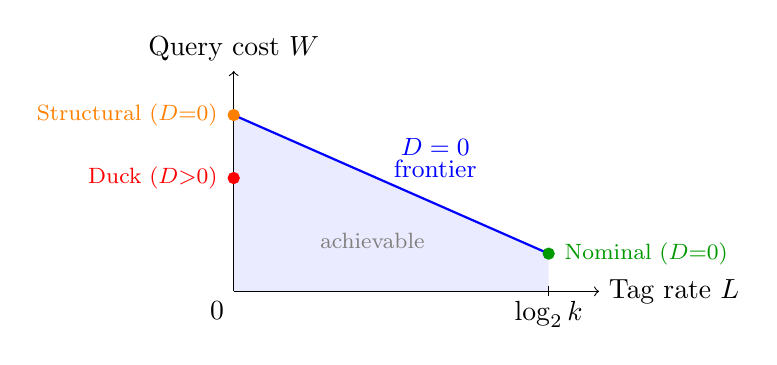
\begin{tikzpicture}[scale=0.8]
  % Shaded D=0 achievable region (draw FIRST)
  \fill[blue!8] (0,0) -- (5,0) -- (5,0.6) -- (0,2.8) -- cycle;

  % D=0 Pareto frontier
  \draw[thick, blue] (0,2.8) -- (5,0.6);

  % Axes (draw after shading)
  \draw[->] (0,0) -- (5.8,0) node[right] {Tag rate $L$};
  \draw[->] (0,0) -- (0,3.5) node[above] {Query cost $W$};

  % Axis labels
  \node[below left] at (0,0) {$0$};
  \node[below] at (5,0) {$\log_2 k$};
  \draw (5,0.08) -- (5,-0.08);

  % Region labels
  \node[blue] at (3.2,2.3) {\small $D = 0$};
  \node[blue] at (3.2,1.95) {\small frontier};
  \node[gray] at (2.2,0.8) {\footnotesize achievable};

  % Points on the D=0 frontier
  \filldraw[orange] (0,2.8) circle (2.5pt);
  \node[orange, left] at (-0.1,2.8) {\footnotesize Structural ($D{=}0$)};

  \filldraw[green!60!black] (5,0.6) circle (2.5pt);
  \node[green!60!black, right] at (5.1,0.6) {\footnotesize Nominal ($D{=}0$)};

  % Duck typing: below frontier, accepts D>0
  \filldraw[red] (0,1.8) circle (2.5pt);
  \node[red, left] at (-0.1,1.8) {\footnotesize Duck ($D{>}0$)};

\end{tikzpicture}
\caption{Schematic illustration of the $(L, W, D)$ tradeoff. For a concrete example with $k = 1000$ classes and distinguishing dimension $d = 10$, the nominal-tag strategy achieves $L = 10$ bits, $W = O(1)$, $D = 0$, while the interface-only strategy requires $W = 10$ queries and incurs $D > 0$ due to attribute collisions.}
\label{fig:lwd-tradeoff}
\end{figure}

The Lean 4 formalization (Appendix~\ref{sec:lean}) provides a machine-checked proof of Pareto optimality for nominal-tag observers in the $(L, W, D)$ tradeoff.

\begin{remark}[Programming language instantiations]
In programming language terms: \emph{nominal typing} corresponds to nominal-tag observers (e.g., CPython's \texttt{isinstance}, Java's \texttt{.getClass()}). \emph{Duck typing} corresponds to interface-only observers (e.g., Python's \texttt{hasattr}). \emph{Structural typing} is an intermediate case with $D = 0$ but $W = O(n)$.
\end{remark}

\begin{remark}[Structural-typing cost parameter]
Using the notation above, a structural check that traverses $s$ members/fields has $W = O(s)$ with $s \le n$.
\end{remark}


% Notation: $n := |\mathcal{I}|$ is the ambient attribute universe size; $s$ is the number of members actually traversed in a structural check (so $s \le n$).
\begin{remark}[Structural-check cost parameter]
When structural typing checks traverse $s$ members/fields (rather than ranging over the full attribute universe), the natural bound is $W = O(s)$ with $s \le n$.
\end{remark}

\noindent Using the notation above, a structural check that traverses $s$ members/fields has $W = O(s)$ with $s \le n$.

% Notation: $n := |\mathcal{I}|$ is the ambient attribute universe size; $s$ is the number of members actually traversed in a structural check (so $s \le n$).
\begin{remark}[Structural-check cost parameter]
When structural typing checks traverse $s$ members/fields (rather than ranging over the full attribute universe), the natural bound is $W = O(s)$ with $s \le n$.
\end{remark}
